
\section{Architecture Integration}

\subsection{Model Support}

\begin{table}[H]
\centering
\small
\begin{tabular}{llllll}
\toprule
\textbf{Architecture} & \textbf{Attention} & \textbf{Nested?} & \textbf{RoPE?} & \textbf{GQA?} & \textbf{FASA pruning?} \\
\midrule
DistilBERT & \texttt{MultiHeadSelfAttention} & No & No & No &  \\
RoBERTa & \texttt{BertSelfAttention} & Yes & No & No &  \\
GPT-2 & \texttt{GPT2Attention} & No & No & No & (causal) \\
Qwen3.5 & \texttt{Qwen3Attention} & No & Yes & Yes & (causal) \\
\bottomrule
\end{tabular}
\end{table}

\subsection{Weight Transfer}

\subsubsection{GPT-2 Conv1D}

\begin{lstlisting}
c\_w = src.c\_attn.weight.data
is\_conv1d = "Conv1D" in cls\_name or c\_w.shape[0] \textless{} c\_w.shape[1]
if is\_conv1d:
    c\_w = c\_w.t()
q\_w, k\_w, v\_w = c\_w.chunk(3, dim=0)
\end{lstlisting}

\subsubsection{RoBERTa Nested}

\begin{lstlisting}
q\_w = src.self.query.weight.data
k\_w = src.self.key.weight.data
v\_w = src.self.value.weight.data
o\_w = src.output.dense.weight.data
\end{lstlisting}

\subsubsection{DistilBERT Flat}

\begin{lstlisting}
q\_w = src.q\_lin.weight.data
# ... etc
\end{lstlisting}

\subsubsection{GQA Handling (Qwen)}

For the K/V projections with $H_{kv} < H$:

\begin{lstlisting}
if src\_out == out\_d:
    target\_w.data.copy\_(w\_oriented)
elif src\_out \textgreater{} out\_d and src\_out \% out\_d == 0:
    rep = src\_out // out\_d
    target\_w.data.copy\_(w\_oriented.view(out\_d, rep, -1).mean(dim=1))
elif src\_out \textless{} out\_d and out\_d \% src\_out == 0:
    rep = out\_d // src\_out
    target\_w.data.copy\_(w\_oriented.repeat(rep, 1))
\end{lstlisting}

This handles GQA pooling (mean) or expansion (repeat) as needed.

\subsection{Injection Algorithm}

\textbf{Algorithm 2:} Inject FASA
\begin{lstlisting}
Input:  layer  , config, old\_attn
Output: new attention in  

1: new $\leftarrow$ MixAttentionMoSKA(config, old=old\_attn, fasa\_keep\_ratio=r)
2: if copy\_weights fails: return None
3: if   has .attention.self:
4:      .attention.self $\leftarrow$ new; is\_nested $\leftarrow$ True
5: elif   has .self:  .self $\leftarrow$ new; is\_nested $\leftarrow$ True
6: elif   has .self\_attn:  .self\_attn $\leftarrow$ new
7: elif   has .attn:  .attn $\leftarrow$ new
8: return new
\end{lstlisting}

\subsection{Masking}

For the pruned path, the padding mask is gathered:

\begin{lstlisting}
pruned\_mask = mask\_2d.gather(1, idx)
\end{lstlisting}

For the causal path, the padding mask is applied directly to the full 
attention.

\subsection{Nested Encoder Detection}

\begin{lstlisting}
has\_out = any(hasattr(src, x) for x in ["dense", "out\_proj", "out\_lin", "c\_proj", "o\_proj"])
is\_nested = cls\_name in ["BertSelfAttention", "RobertaSelfAttention", ...]
if hasattr(src, "self") and hasattr(src, "output"):
    is\_nested = True
\end{lstlisting}

\subsection{Registry}

\begin{lstlisting}
@ATTENTION\_REGISTRY.register("fasa")
@ATTENTION\_REGISTRY.register("fasa\_attention")
@ATTENTION\_REGISTRY.register("mixattention\_moska")
class MixAttentionMoSKA(BaseAttention):
    ...
\end{lstlisting}

\subsection{Common Pitfalls}

\subsubsection{Decoder Path is a No-Op}

For GPT-2, FASA does \textbf{no pruning}. Users expecting speedup should be 
aware.

\subsubsection{Pruning Every Forward Pass}

The importance score is recomputed every forward pass. This means the 
selected $\mathcal{S}$ changes between calls on the same input if batch 
composition changes. Not a bug, but worth documenting.

\subsubsection{`attention\_mask` Fallback}

\begin{lstlisting}
mask = kwargs.get("mask", None)
if attention\_mask is None and mask is not None:
    attention\_mask = mask
\end{lstlisting}

Silent fallback. Not harmful but non-obvious.
\begin{lstlisting}

---
\end{lstlisting}

\begin{figure}[H]
\centering
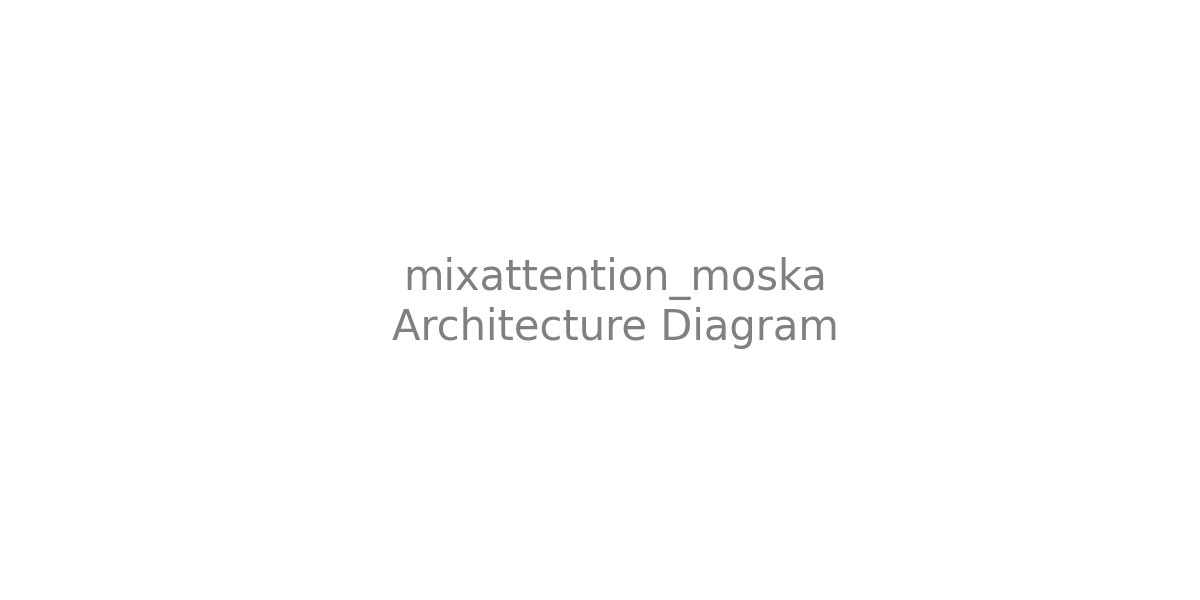
\includegraphics[width=\linewidth]{figures/architecture.png}
\caption{High-level architectural diagram of mixattention\_moska.}
\label{fig:arch_mixattention-moska}
\end{figure}

